\chapter{A Single Stage PV System}\label{ch:system_description}
\section{The System}
The system is shown in \Vref{fig:sys_gram} and can be divided into three major parts, solar panel/cells, H-bridge, controller and  LCL filter. The transformer is optional depending on local rules and regulations. In some countries, it is compulsory to add the transformer for the purpose of isolation and protection, while in some countries it is not required. It is allowed to have transformerless system in Australia according to regulations\cite{ASNZS-5033-2014}. The whole system design is fairly simple and straightforward. 
\begin{figure}[!b]
\centering
    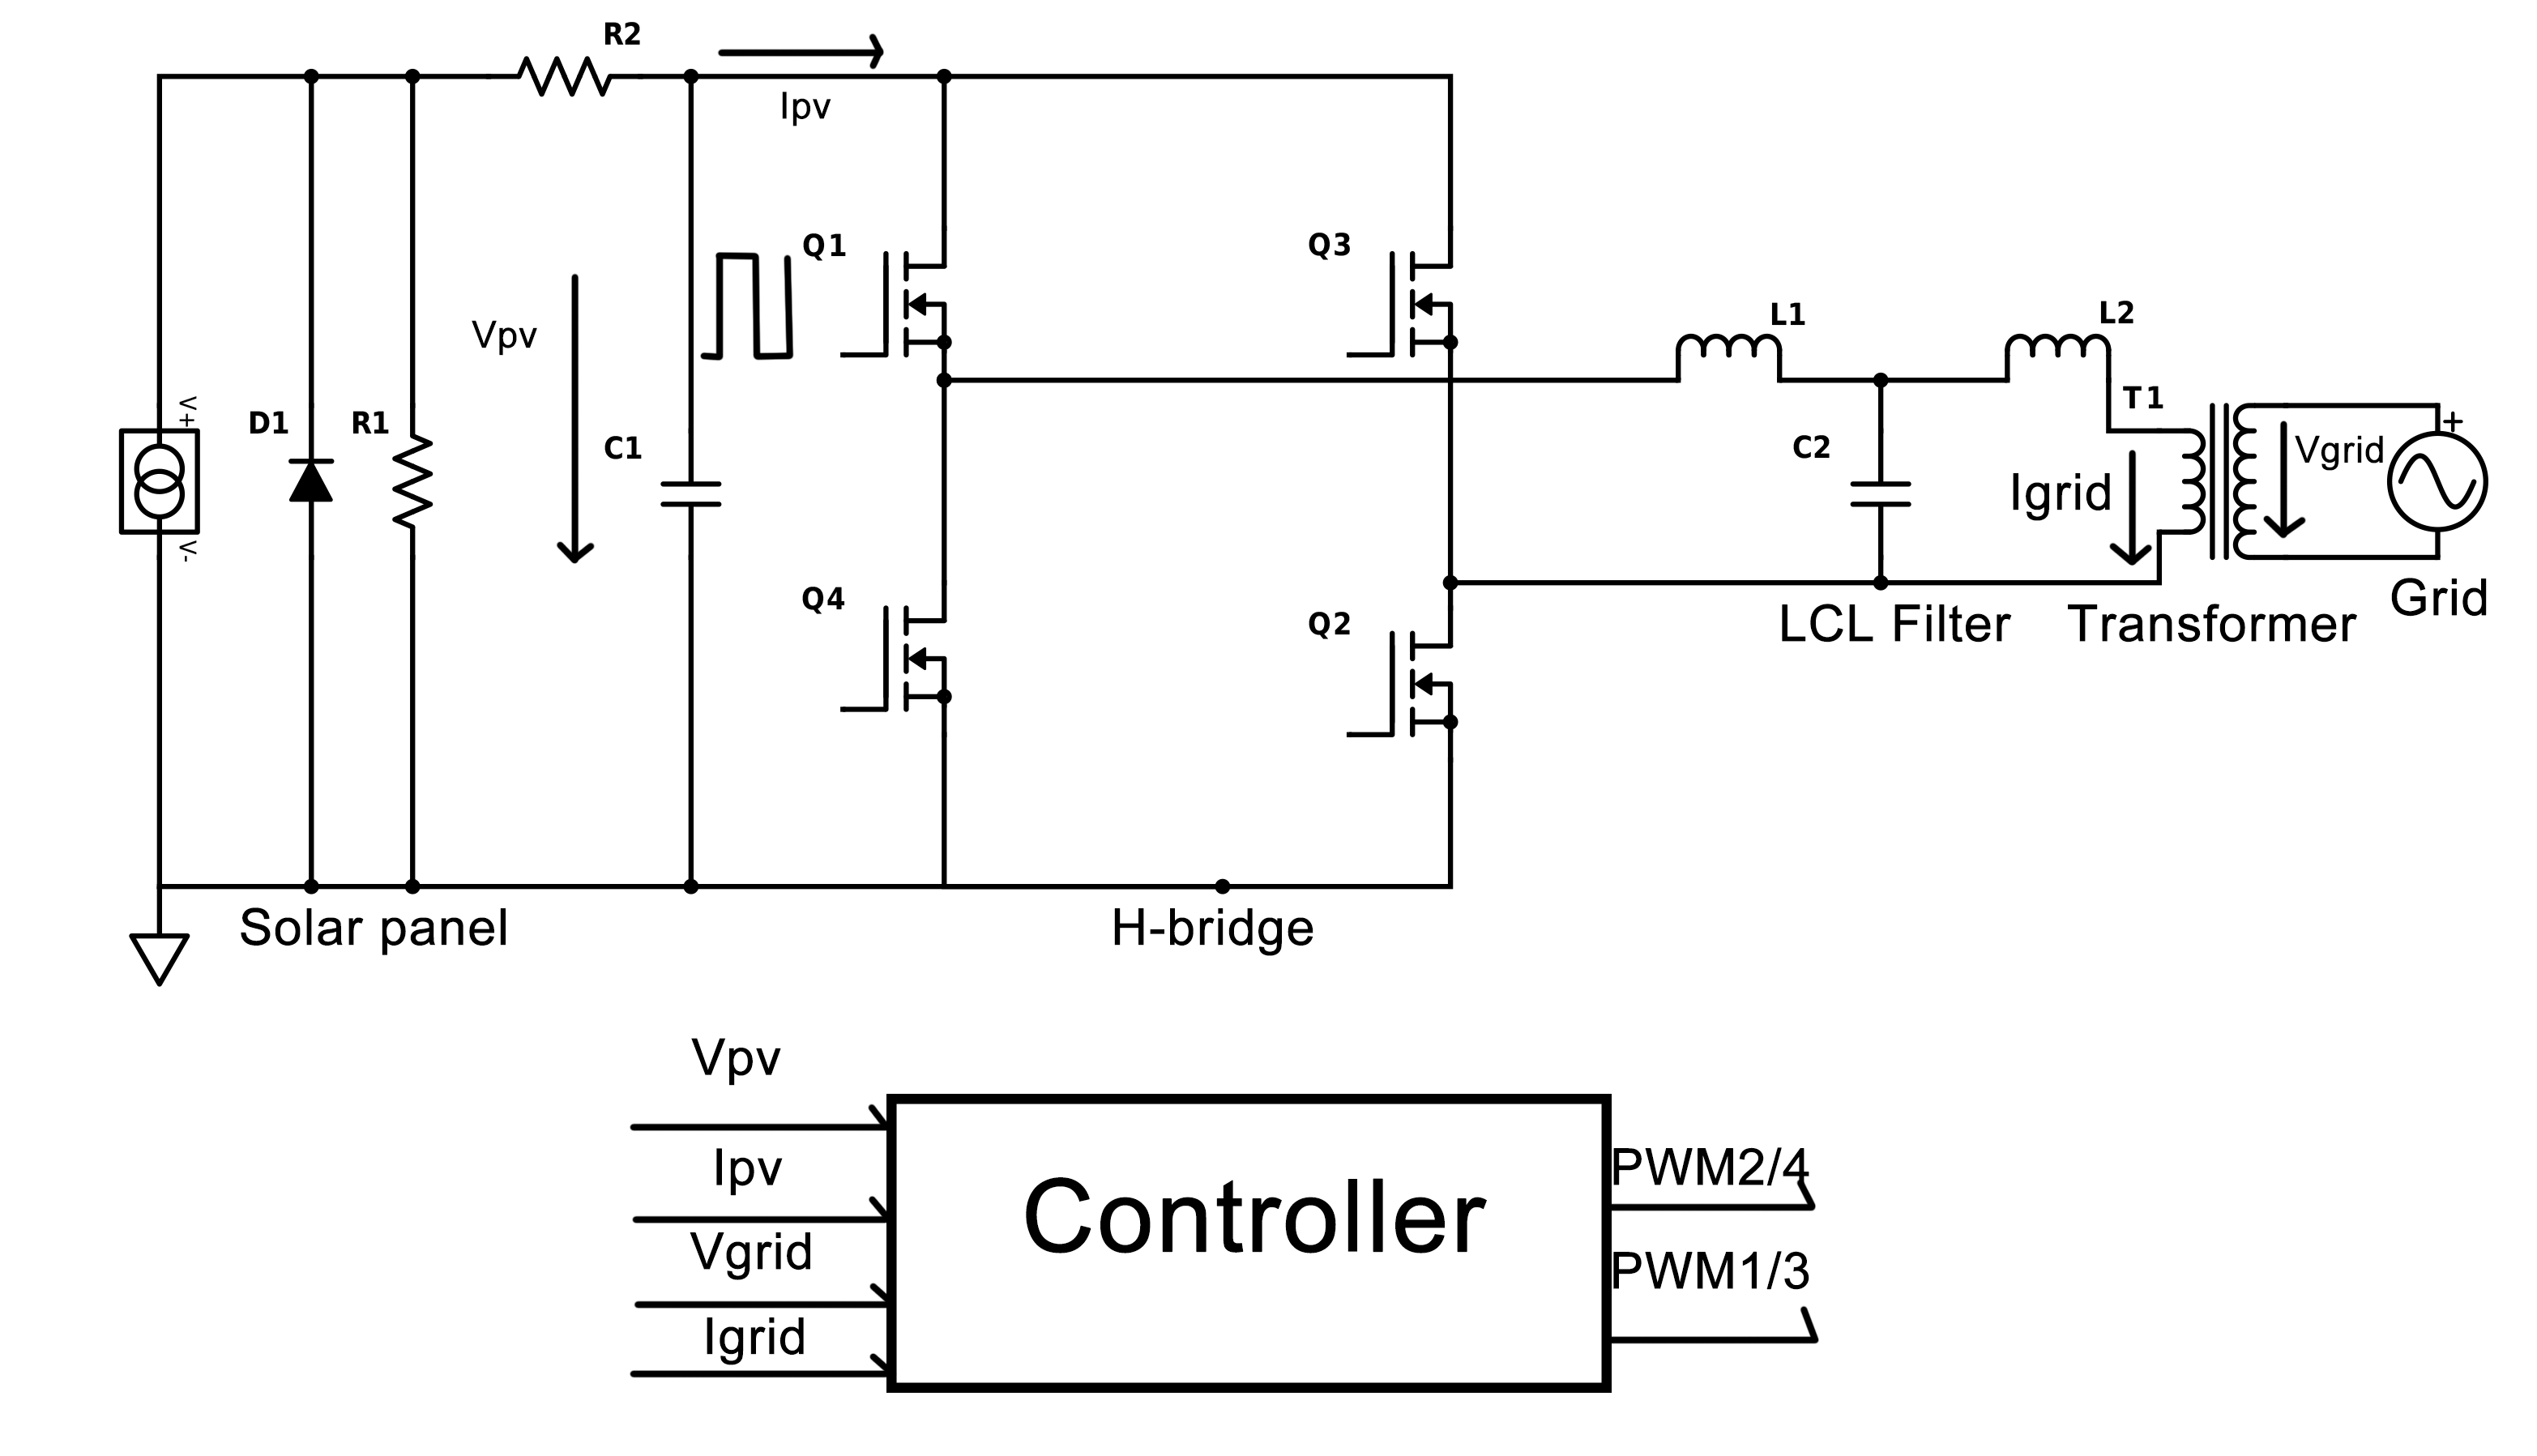
\includegraphics[width = 1\textwidth]{figures/system_diagram.png}
    \caption{A single stage grid-connected PV system}
    \label{fig:sys_gram}	
\end{figure}
Detailed description on solar cell model can be found in section \ref{sec:solar_cell}. 

\section{Modeling of Solar Cell}\label{sec:solar_cell}
\begin{figure}[b]
\begin{minipage}{.5\textwidth}
    \centering
    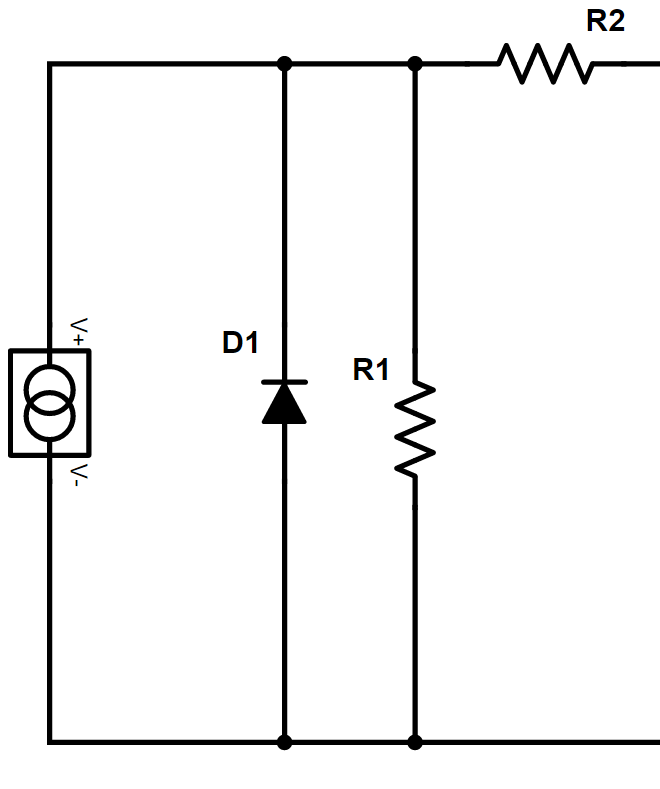
\includegraphics[width = 0.5\textwidth]{figures/cell_equal.png}
    \caption{Equivalent circuit of single solar cell}
    \label{fig:cell equivalent}	
\end{minipage}
\begin{minipage}{.5\textwidth}
    \centering
    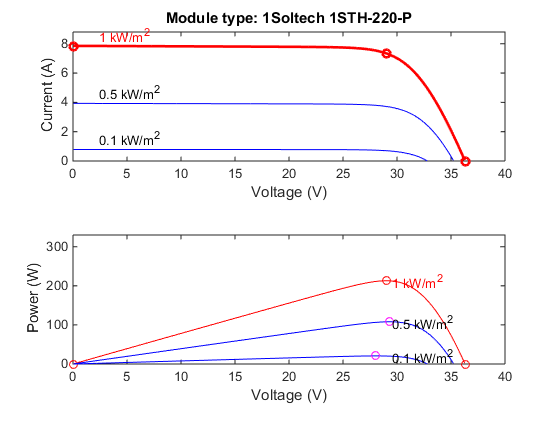
\includegraphics[width = 0.75\textwidth]{figures/typical_solar.png}
    \caption{Output characteristic with different sunlight}
    \label{fig:typical solar module}	
\end{minipage}
\end{figure}
There are lots of solar cell models existed so far and the most widely used model is presented here. The equivalent circuit of a single solar cell is shown in \Vref{fig:cell equivalent}. It is composed of a photo-generated current source, a parallel connected diode, a shunt resistor and a series connected resister\cite{wenham2007applied}. In present of parasitic resistors, the solar cell output characteristic can be represent be the following equations\cite{RN24}\cite{RN26}. 
\begin{eqnarray}\label{equ:solar cell}
    I = I_L - I_o(e^{\frac{V+IR_2}{(\frac{nkT}{q})}} - 1) - \frac{V+IR_2}{R_1}
\end{eqnarray}
In this equation, $I$ is the output current which flows out of the solar cell for positive value. It is possible produce negative current which is equivalent to current flows into cells, however, this situation should be avoided because .  $V$ is the terminal voltage of the cell. $I_o$ is the parallel dido saturation current. $I_L$ is the light generated current. $n$ is the number of cells in series. $q$ is the elementary charge. $T$ is the current ambient temperature of the cell. Equation \eqref{equ:solar cell} indicates that when the terminal voltage is low, almost all the current can flow out of the cell. When the voltage goes higher, the saturation current of the parallel diode begin to increase, thus reducing the output current. Eventually the output current can go to zero as the increasing of terminal voltage. 

Temperature can affect the output characteristic of the solar cell as well, since under different temperature condition, electron have different electron mobility. Generally, the higher the temperature, the higher is saturation current of parallel connected diode, thus leading to the decreasing of total output power. \Vref{fig:typical solar module_temp} illustrate a solar panel ouput characteristic with respect to various temperature. 

The solar panel on the market usually consist of multiple solar cells connected in series or in parallel to increase the terminal open circuit voltage or maximum short circuit current. A typical output characteristic of a solar panel module is shown in \Vref{fig:cell equivalent}. Due to the output characteristic of solar cell, there exist a maximum power point which have been marked in the figure with a red circle. If we want to extract the most power out of the panel or cells, \gls{MPPT} algorithm is needed to archive this goal.
\begin{figure}[t]
    \begin{minipage}{.5\textwidth}
            \centering
            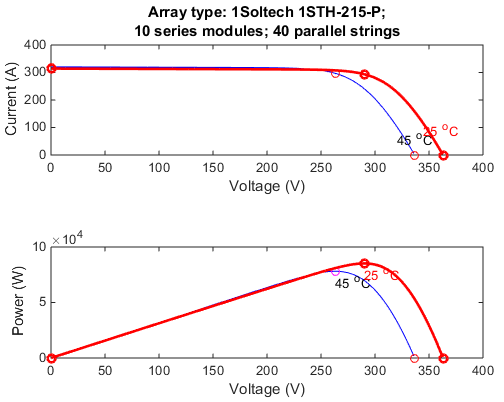
\includegraphics[width = 0.8\textwidth]{figures/typical_solar_temp.png}
            \caption{Output characteristic with different temperature}
            \label{fig:typical solar module_temp}
    \end{minipage}
    \begin{minipage}{.5\textwidth}
        \centering
        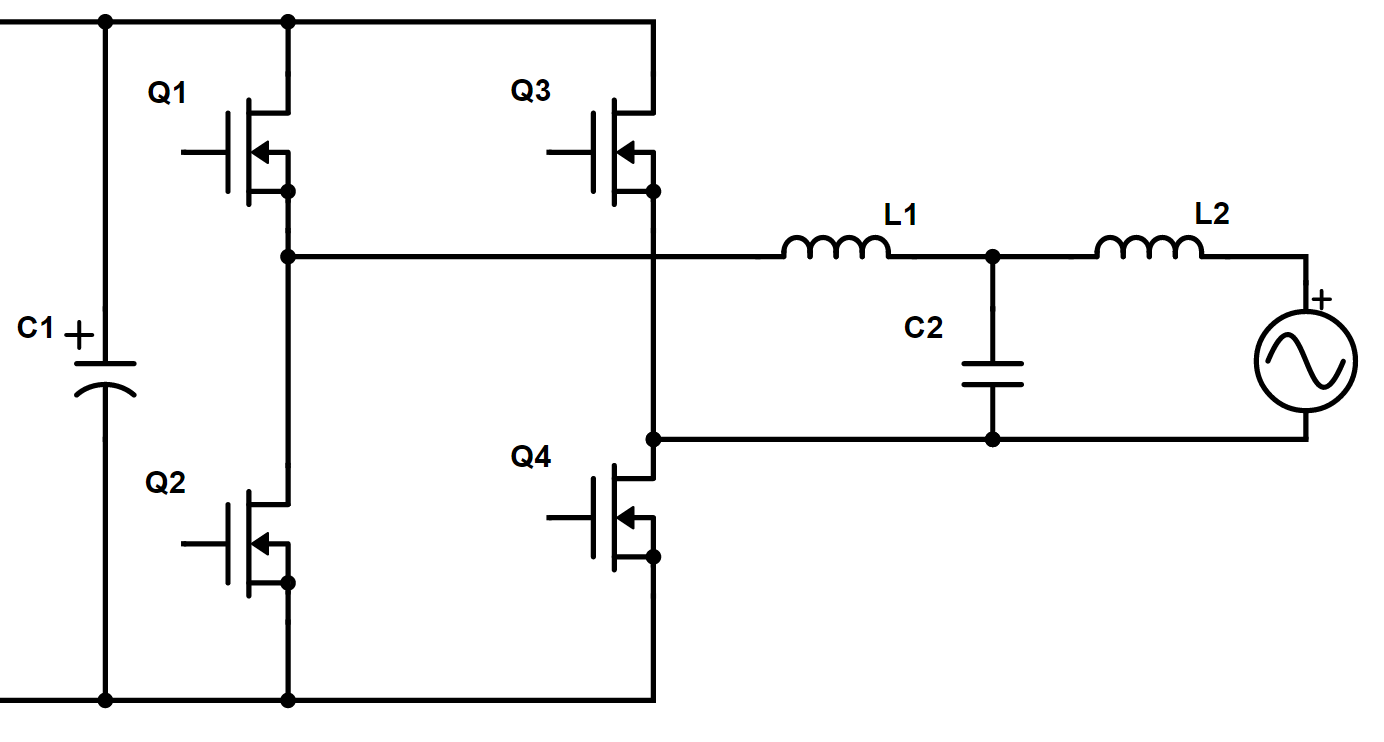
\includegraphics[width = 1\textwidth]{figures/topology.png}
        \caption{H-bridge with LCL filter}
        \label{fig:topology}
    \end{minipage}
\end{figure}

\subsection{MPPT}
As mentioned before, \gls{MPPT} is a method for extracting the most power out of solar cell. \gls{MPPT} have been studied by many researchers many algorithms have been proposed, such as \gls{PO}, \gls{IC}\cite{RN16}\cite{RN34}\cite{RN28}\cite{RN12}\cite{RN18}. \

\gls{PO} also known as "hill climbing" method, is one of the most classic and simple algorithm and have been widely used in many \gls{PVS}. The method actively adjust the output voltage of the connected solar panel by a small amount $\Delta V$ and sense the ouput current to calculate the resulted change in output power $\Delta P$ by substrate current power with previous power. If $\Delta P$ is greater than zero, it means that output voltage may be set higher to gain more power. If $\Delta P$ is less than zero, it means that MPP has been passed and output voltage needed to be reduce. The power trajectory moves like climbing up a "mountain" which is the maximum power archivable under current sunlight condition. the whole algorithm can be described in \Vref{fig:hill_climb}.
\begin{figure}[!b]
\centering
    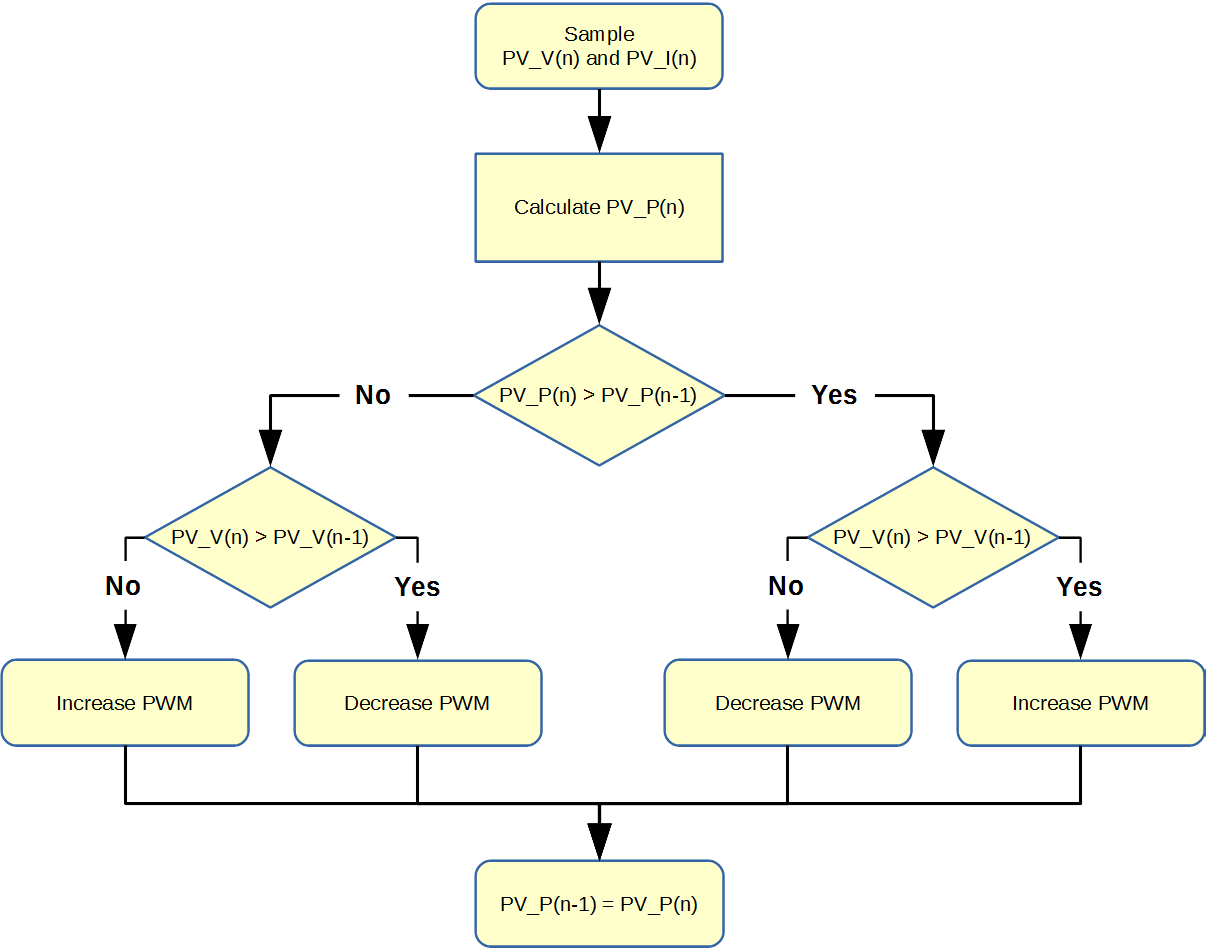
\includegraphics[width = 1\textwidth]{figures/pando.png}
    \caption{P\&O Algorithm}
    \label{fig:hill_climb}	
\end{figure}

The problem with \gls{PO} method is the adjustment of power output based on perturb. The algorithm tries hard to get close to the maximum power point instead of staying at the maximum power point, of which lead to compromise of system efficiency. The system may operate around MPP depending on the size of perturb. Large perturb may lead to fast response when irradiance is changing dynamically but largely compromised steady state efficiency. Small perturb may result in high steady state efficiency, however, the algorithm may have little transient performance. 

\subsection{H-bridge and PWM}

There are lots of different types of circuit topologies for inverter applications\cite{7392067}\cite{7356292}, but the simplest one is classical H-bridge configuration. \Vref{fig:topology} shows a simple H-bridge with LCL filter configuration which would be used in the later simulation.

H-bridge, in this case, has four switching components which are represent by the symbol of MOSFET. By turning on and off the switching, three different levels of voltage can be sense from output terminals which are $\pm V_{dc}$ and zero. The state of the switches are controlled by desired \gls{PWM} signals to generate desired voltage levels at between switching intervals.

\gls{PWM} is particular important for success of converting \gls{DC} to \gls{AC}. \gls{PWM} is a modulation technique to encode signal or signals into a pulse train. There exists two different types of modulation technique for a classic four switches H-bridge, bipolar and unipolar modulation for solar \gls{PV} applications. The difference between the two is that in bipolar modulation, the output voltage can only be either $\pm V_{dc}$ compared with unipolar modulation. With one additional voltage level, unipolar modulation can produce higher efficiency and lower TOTAL Harmonic Distortion(THD). 

One issue related with \gls{PVS} is common mode voltage which usually cannot be found in other applications of \gls{DC} to \gls{AC} inverters. Since usually \gls{PV} panels are mounted on large plates of mental, voltage potential difference, also known as common mode voltage between panels and ground,  can build up due to capacitor effect leading to malfunctioning of circuit breaker at the grid side. One way to get around this issue is to use bipolar \gls{PWM} if a H-bridge configuration is used. The reason why unipolar may suffer the issue is that when all the switches are turned off, the output terminals are flouting with respect to ground, thus lead to common mode voltage building up at the terminals. When the switches are turn on, closed circuit loop can be create with protection devices on grid side connected to earth ground. Anther way to get around the issue is to use the different inverter topologies to isolate panels and converter. One good example of such configuration proposed by this paper\cite{7356292}.

There is a limitation on the \gls{SSGPVC} which is the voltage rating. The voltage on the input side need to be higher than the output voltage which means the overall voltage gain of H-bridge is always less than one. Interfacing with high voltage grid would results in large number of \gls{PV} panels or cells connected in series on the input side to build up the voltage. 

\section{LCL Filter}

As shown in \Vref{fig:topology}, the circuit make use of a filter which is consist of two inductors and one capacitor. High frequency modulation signal requires a proper filter to eliminate any undesired high frequency harmonics to fulfill the requirement imposed by THD. The filter is a high orders passive filter which has superior performance compared with traditional single inductor filter in terms of harmonic elimination. However, high order filters are more difficult to control, it's resonance frequency can cause stability issue if not carefully deal with\cite{RN15}.

\subsection{Grid Synchronization}
\gls{AC} voltage generated by the inverter should have identical phase with the grid voltage so that there is not cancellation of voltage which might cause instability of the grid. In order to archive synchronization with the grid, \gls{PLL} is used. The \gls{PLL} served as a servo system controlling the signal phase of its output. The performance of it has a direct impact on control loop of grid-connected power applications. It should be able to reject source of errors including voltage unbalance, line notching, line dip, frequency jump. The most critical thing is to keep maintaining a clean and reliable phase lock to grid voltage. There are lots of \gls{PLL} structures designed for various applications. 

Among those \gls{PLL} structures, \gls{SOGI} have been widely discussed and used in many \gls{PVS}. It can be selectively tuned to eliminate other frequency components other than grid frequency and its nominal frequency would not be affected by the frequency change\cite{RN12}. The basic structure of \gls{SOGI} is shown in \Vref{fig:SOGI}.
\begin{figure}[t]
     \centering
     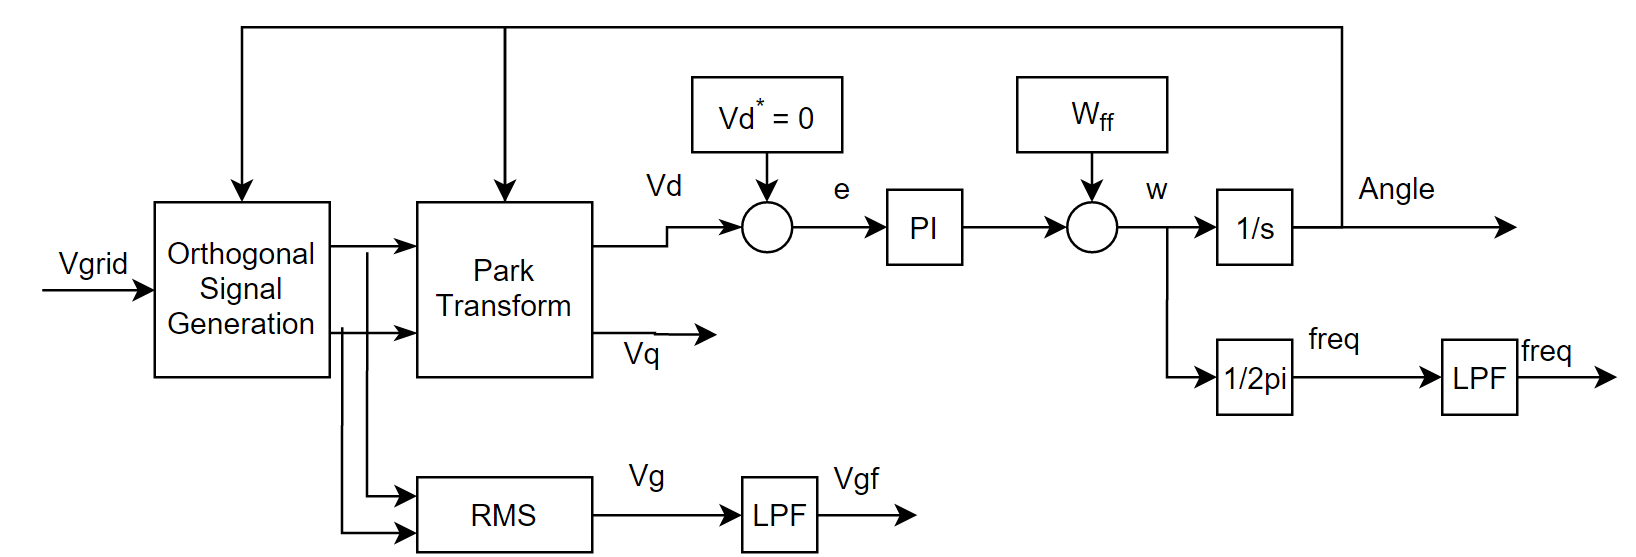
\includegraphics[width = 0.8\textwidth]{figures/SOGI.png}
     \caption{Basic structure of SOGI}
     \label{fig:SOGI}
\end{figure}

\subsection{Feedback Control}
\begin{align}\label{equ:pi}
    T(s) = K_p + \frac{K_i}{s}
\end{align}
\begin{align}\label{equ:pr}
    T(s) &= K_p + \frac{K_i}{s^2 + \omega_1^2}
\end{align}
\begin{align}\label{equ:compensator}
    C(s) &= \sum\limits^{k}_{n=3, 5, 7}\frac{K_n}{s^2+\omega_n}
\end{align}
For current control of \gls{SSGPVC}, \gls{PI} and \gls{PR} are common choices. The transfer function of a typical \gls{PI} is illustrated in Equation \eqref{equ:pi}. In a negtive feedback system, \gls{PI} can be used to eliminate error between target and output value. The proportional term may help reduce the error quickly and the integral term may be used to eliminate steady state error. It features simplicity as well as reliability and has been used widely in many control engineering applications. Since \gls{PI} is a first order system, the performance to track a sinusoidal target is actually not very great and the error cannot be eliminated. It also suffers poor high frequency components rejection performance.

Equation \eqref{equ:pr} represents \gls{PR} where $\omega_1$ is the fundamental frequency of the grid in radiance. $\omega_1$ is either $50\times 2\pi=314.16$ rad/s for 50 Hz system or $377$ rad/s for 60 Hz system. Equation \eqref{equ:compensator} represents harmonic compensators for output current where $\omega_n$ are harmonics. Typically in a \gls{PVS}, both \gls{PR} and compensator are used in conjunction to archive better performance. One good aspect offered by the compensator is that harmonics can be selectively eliminated by varying $\omega_n$ where $\omega_n = n \times \omega_1$ and $n=3,5,7\dots$. The downside of the compensator is that it may result in high orders system which requires more computation power that some low end microcontrolers may struggle to offer. 

\section{Opal-RT Simulator}
\begin{figure}[b]
     \centering
     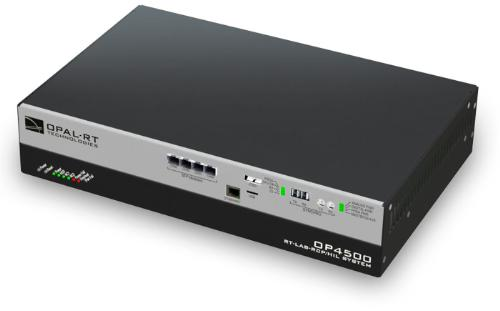
\includegraphics[width = 0.5\textwidth]{figures/op4500.jpg}
     \caption{OP4500 \gls{RT} simulator}
     \label{fig:op4500}
\end{figure}
Opal-RT is a company based in Canada which provide \gls{RT} simulators and its software solutions to make \gls{RT} simulation possible. In this project, their simulator model OP4500 which is shown in \Vref{fig:op4500} is used. OP4500 combine traditional X86 architecture and latest \gls{FPGA} simulation technique to accelerate the process. The onboard Intel CPU can archive minimum time step of 7 $\mu
$s without getting overrun and \textit{eHS} \gls{FPGA} based simulation solver is able to archive minimum time steps of 250 ns. It also multiple Input and Output(IO) modules including both analog and digital types, for interfacing external hardwares to perform \gls{HIL} simulation. The simulartor can be either a controller to run control algorithm and generate desired signal to control actual hardwares or become a simulated plant to develop and verify functionalities of external controller. 

\textit{RTLAB} is the software running inside a host personal computer(PC) in order to be able to use the box for simulations. \textit{RTLAB} currently is fully compatible with \textit{MATLAB} and \textit{SIMULINK} which make it easy to develop models for \gls{RT} simulation. currently, \textit{RTLAB} only supports up to \textit{MATLAB 2014B} and not all models in \textit{SIMULINK} are supported. 


